  \documentclass[journal,12pt,twocolumn]{IEEEtran}
\usepackage[none]{hyphenat}
\usepackage{enumitem}
\usepackage{graphicx}
\usepackage{listings}
\usepackage{kvmap}
\usepackage[utf8]{inputenc}
\usepackage{hyperref}

\usepackage{caption}

\title{IDE  \\ \textbf{\\JOHNSON COUNTER}}
\author{Manoj Chavva- FWC22055}

\begin{document}
\maketitle

\tableofcontents
\vspace{0.5cm}
\begin{abstract}
  This Manual shows the design and Implemantation of four bit Johnson counter with 7474 IC's.
\end{abstract}   


 
     \section{Components}  
       

\begin{tabular}{|c|c|c|}
    \hline 
      \textbf{S.No} & \textbf{Component} & \textbf{Number}\\
      \hline
	1. & Arduino & 1 \\
	2. & Bread Board & 1 \\
	3. & Jumper Wires(M-M) & Required \\
	4. & LED & 4 \\
	5. & 7474 & 2\\
      \hline
      
   \end{tabular}
   

     \vspace{0.35cm}




\section{Introduction}
\begin{enumerate}
  \item Johnson counters are used to store or process or count the number of events occurred within the circuit.
  \item It is designed with a group of flip-flops, where the inverted output from the last flip-flop is connected to the input of the first flip-flop.
  \item In Johnson counter
  \\No. of states = No. of flip-flop used  
\\Number of used states=2n  
\\Number of unused states=2n - 2*n  
\item Generally, it is implemented by using D flip-flops or JK flip-flops. 
Here, It is implemented by D flip-flop.
\end{enumerate}

    \vspace{2.5cm}   



\section{Circuit Diagram}
\begin{enumerate}
\item The inverted output of the last flip-flop ‘$\bar{Q}$n’ is fed back to the first flip-flop in the sequence bit pattern. 
\item The counter registers cycles in a closed-loop i.e circulates within the circuit.
\begin{figure}[h]
    \centering
    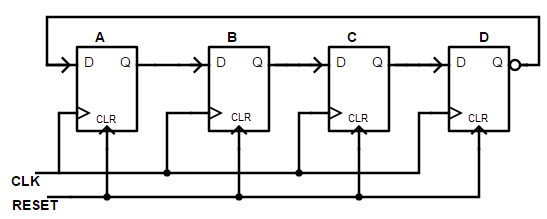
\includegraphics[width=8cm, height=4.2cm]{counter.jpg}
    
    \caption{Four bit Johnson Counter}

\end{figure}
\item Reset pin acts as an on/off switch. So, the flip-flops can be enabled by clicking the Reset switch.

\item CLK pin is used to observe the changes in the output of the flip-flops.
\end{enumerate}



\section{Procedure}
\begin{enumerate}
\item Connect the two 7474 IC's, LED's and Aurdino according to table \ref{table:1}
\item Observe the states of LED and verify the truth table using the code from the link.



\end{enumerate}

\begin{figure}[h]
\centering
    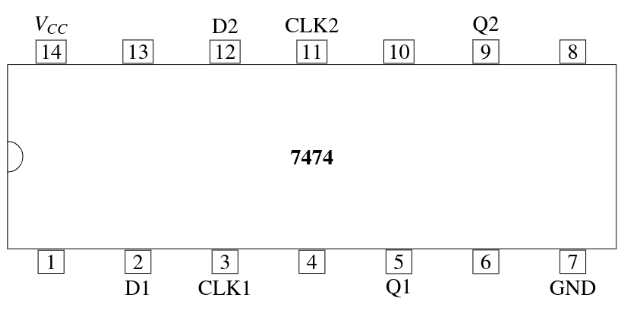
\includegraphics[width=5cm, height=3cm]{7474.png}
    
    \caption{7474 IC}

\end{figure}

\newpage

\begin{table}[h]
\large
\centering
\begin{tabular}{|l|}
\hline

\url{https://github.com/ManojChavva/FWC/blob/main/IDE/JohnsonWithIC/code.cpp} \\
\hline

\end{tabular}

\end{table}


\begin{table}[h]
\large
\centering

\begin{tabular}{|l|l|l|l|l|l|l|l|l|l|llll|ll|}
\hline
\textbf{Arduino} &   &      &      &      &   &      &      &      & GND & \multicolumn{4}{l|}{Vcc}                                                       & \multicolumn{2}{l|}{ClK  13} \\ \hline
\textbf{7474}    & 2 & 2,5  & 5,12 & 12,9 & 9 &      &      &      & 7   & \multicolumn{1}{l|}{14} & \multicolumn{1}{l|}{1} & \multicolumn{1}{l|}{4} & 10 & \multicolumn{1}{l|}{3}  & 11 \\ \hline
\textbf{7474}    & 8 &      &      &      & 2 & 2,5  & 5,12 & 12,9 & 7   & \multicolumn{1}{l|}{14} & \multicolumn{1}{l|}{1} & \multicolumn{1}{l|}{4} & 10 & \multicolumn{1}{l|}{3}  & 11 \\ \hline
\textbf{LED}     &   & LED1 &      & LED2 &   & LED3 &      & LED4 &     & \multicolumn{1}{l|}{}   & \multicolumn{1}{l|}{}  & \multicolumn{1}{l|}{}  &    & \multicolumn{1}{l|}{}   &    \\ \hline
\end{tabular}

\caption{Connection Table.}
\label{table:1}
\end{table}






 



% Define block styles
\tikzstyle{decision} = [diamond, draw, fill=blue!20, 
    text width=4.5em, text badly centered, node distance=3cm, inner sep=0pt]
%\tikzstyle{block} = [rectangle, draw, fill=blue!20, 
%    text width=5em, text centered, rounded corners, minimum height=4em]
\tikzstyle{block} = [rectangle, draw, 
    text width=5em, text centered, rounded corners, minimum height=4em]

\tikzstyle{line} = [draw, -latex']
\tikzstyle{cloud} = [draw, ellipse,fill=red!20, node distance=3cm,
    minimum height=2em]
    
\begin{tikzpicture}[node distance = 3cm, auto]
    % Place nodes
    \node [block] (init) {Arduino};
   
    \node [block, below of=init, node distance = 4cm] (identify) {Flip Flops};
    \node [block, below of=identify ] (evaluate) {LED's};
	\node at (4,-2)[block] (delay) {Delay};
\begin{scope}[->,>=latex]
    \foreach \i in {-3,-1,1,3}
    { 
      \draw[->] ([xshift=\i * 0.2 cm]delay.north) |- ([yshift=\i * 0.2 cm]init.east) ;
      \draw[->] ([xshift=\i * 0.2 cm]init.south) -- ([xshift=\i * 0.2 cm]identify.north) ;
       \draw node at (\i * 0.2,-2+\i * 0.2) { \textbullet} ;
       \draw[->] (\i * 0.2,-2+\i * 0.2) -- ([yshift=\i * 0.2 cm]delay.west) ;
      
    }
\foreach \i in {-2,...,1}
    { 
      \draw[->] ([xshift=\i * 0.35 cm]identify.south) -- ([xshift=\i * 0.35 cm]evaluate.north) ;
    }
\foreach [count=\i] \j in {1,2,3,4}{
            \node (\i) at ( 0.8-\i * 0.35, -5.5) {\j} ;
            }
\foreach [count=\i] \j in {Q1,Q2,Q3,Q4}{
            \node (\i) at ( 0.5-\i * 0.4, -1.0-\i*0.4) {\j} ;
            }

\foreach [count=\i] \j in {D1, D2, D3, D4}{
            \node (\i) at ( 1.6, 1.2-\i*0.4) {\j} ;
            }
    
\end{scope}

    
   
\end{tikzpicture}

\centering Fig: 3 Sequential Circuit



\section{Truth Table}



\begin{center}
    
    \setlength{\arrayrulewidth}{0.5mm}
\setlength{\tabcolsep}{18pt}
\renewcommand{\arraystretch}{1.1}
   
\begin{tabular}{|l|l|l|l|l|l|l|l|l|}
\hline
\textbf{CLK} & \textbf{D1} & \textbf{D2} & \textbf{D3} & \textbf{D4} & \textbf{Q1} & \textbf{Q2} & \textbf{Q3} & \textbf{Q4} \\ \hline
0            & 0           & 0           & 0           & 0           & 0           & 0           & 0           & 0           \\ \hline
1            & 1           & 0           & 0           & 0           & 1           & 0           & 0           & 0           \\ \hline
2            & 1           & 1           & 0           & 0           & 1           & 1           & 0           & 0           \\ \hline
3            & 1           & 1           & 1           & 0           & 1           & 1           & 1           & 0           \\ \hline
4            & 1           & 1           & 1           & 1           & 1           & 1           & 1           & 1           \\ \hline
5            & 0           & 1           & 1           & 1           & 0           & 1           & 1           & 1           \\ \hline
6            & 0           & 0           & 1           & 1           & 0           & 0           & 1           & 1           \\ \hline
7            & 0           & 0           & 0           & 1           & 0           & 0           & 0           & 1           \\ \hline
\end{tabular}
   
   \vspace{0.5cm}
   \centering Table II: Truth Table.
\label{table:2}
 \end{center}







 
 \section*{Conclusion}
 Thus the Johnson counter designed and Implemented.

\end{document}